\section{Demonstration}
% how to evaluate?

% random picking relation, labeling true or false?
% the count precision@x?

% check: 1. GY's paper
%        2. ritter's paper

% Check their page size
% write about our size.
% and compare the version of MI-Equal, MI-Uniform, TfIdf-Equal, TfIdf-Uniform
In the demonstration part, we first introduce the experimental setup.
Secondly we evaluate the accuracy of relation type inferring.
Then we present our web interface of RvSp system, and finally
we provide some example relations with the inferred argument types.

\subsection{Experimental Setup}
% Add Freebase dump citation
The input ReVerb dataset is released by Lin et al.\shortcite{lin2012entity}, containing 3 millions of relation tuples with high quality.
We observed that an argument is unlikely to be an entity in Freebase, for example:

$\langle Metro\ Manila,\ consists\ of,\ \textbf{12 cities}\rangle$

\noindent
Thus, we remove the tuple if one argument is lowercased and not recognized by SUTime.
After cleaning, the system collects 1,159,644 tuples and 176,235 relation groups.

We use the 16 Feb. 2014 dump of Freebase for our system. In the step of entity linking, we set $\tau$ to be 0.667
as the empirical value.
%1. data come from Rv 3M
%2. Freebase.
% set tau to be 0.667 as the empirical value
%2. lowercased are removed
%3. remaining xxx relations, and xxx tuples.

\subsection{Evaluation Results}
% Important part, how to evaluate ?
For the evaluation task, we randomly pick 100 binary relations from the system.
For each relation, we extract top 20 type pairs.
The test set contains 2,000 $\langle t1,\ rel,\ t2 \rangle$ triples in total.
We assigned 3 human annotators to judge whether $\langle t1,\ t2 \rangle$ is a preferred pair for $rel$.
Based on majority voting, we calculate the average precision of type pairs at rank 5, 10, 15, 20, respectively.
% given rel and a, output b?
% given rel, output all a b?

\tabref{tab:precision} shows that the average precision of type pairs goes down when the rank increases.
At rank=20, the precision can still reach 94.4\%, proving that RvSp can find enough correct type pairs.

\begin{table}[htbp]
	\centering
	\caption{Average Precision at Different Ranks}
	\begin{tabular}{Ic|c|c|c|cI}
		%\toprule
        \whline
		Rank & @5 & @10 & @15 & @20 \\
        \hline
        Precision & 0.958 & 0.955 & 0.948 & 0.944 \\
        \whline
	\end{tabular}%
	\label{tab:precision}%
\end{table}

%\begin{figure%}[htp]
%\centering \scalebox{0.6}{\includegraphics{eval.eps}}
%%\epsfig{file=figure1-cropped.eps, width=2\columnwidth}
%%\scalebox{0.35}
%\caption{Average precision at different ranks.}
%\label{fig:precision}
%\end{figure}

% We randomly sample K relations, use 3 annotators to annotate whether a type pair is true or not.
% count precision@px

\subsection{Web Interface}
We set up a website \footnote{http://202.120.38.146/rvsp} for users to query the schemas of a binary relation.
Figure 2 shows the snapshot of the query interface.
Users can search for type pairs by providing the binary relation alone, the interface will output the ranked type pairs.
Further more, users can enter the binary relation with a Freebase type on either subject or object side, then the interface will show a ranked list of preferred types on the other side.
Before querying, the interface will transform the relation pattern, using the method introduced in section 4.

In RvSp, a type is recognized by Feebase type id, which doesn't match its name exactly. Due to this fact, we provide typing suggestion in the web interface, making users query easier.
When a user inputs a type id, all types containing the input string are displayed.
Users can browse Freebase website \footnote{http://www.freebase.com} for detail information about type id.
\\
\\

\begin{figure}[ht]
\centering
\epsfig{file=cropped-demo1.eps, width=0.6\columnwidth, angle=270}
\caption{Query Interface}
\label{fig:demo1}
\end{figure}


\figref{fig:demo1} shows the result page.
User can click ``page up'' and ``page down'' to check more results.
Besides, for each relation schema, user can click ``detail'' link too check all its support tuples.
The schema details are shown in \figref{fig:demo2}.
\\
\\

\begin{figure}[ht]
\centering
\epsfig{file=cropped-demo2.eps, width=0.6\columnwidth, angle=270}
\caption{Schema Details}
\label{fig:demo2}
\end{figure}

Finally, \figref{tab:sample_relation} shows the example of binary relations, and their schemas.
% we set parameters as: .........
% how to show?? top1, top5, or top10??
As we can see, with a well-defined type hierarchy, RvSp is able to extract both coarse-grained and fine-grained type information from entities, resulting in a informative type lists.

\begin{table*}[htbp]
	\centering
	\caption{Sample Relation Schemas}
	\begin{tabular}{Ic|l|lI}
		%\toprule
        \whline
		Relation & Arg1 Type & Arg2 Type \\
        \whline
        & book.author & book.book \\
        & book.author & book.written\_work \\
        be the writer of & tv.tv\_writer & award.award\_nominated\_work \\
        & people.person & book.book \\
        & people.person & book.written\_work  \\
        \hline
        & fictional\_universe.fictional\_character & tv.tv\_actor  \\
        & fictional\_universe.fictional\_character & film.actor  \\
        be play by & fictional\_universe.fictional\_character & people.person  \\
        & fictional\_universe.fictional\_character & influence.influence\_node  \\
        & people.person & tv.tv\_actor  \\
        \hline
        & organization.organization\_founder & organization, organization \\
        & people.person & organization, organization \\
        found & people.deceased\_person & organization, organization \\
        & organization.organization\_founder & business.business\_operation \\
        & organization.organization\_founder & business.employer \\
        \whline
	\end{tabular}%
	\label{tab:sample_relation}%
\end{table*} 